%!TEX root = ../../Main.tex
\graphicspath{{Chapters/Struktur/}}
%-------------------------------------------------------------------------------

\section{Struktur}

I dette projekt er der taget et valg udfra læringsmålene om at vi bruger Blackfin platformen til at udføre projektetes funktionalitet. Da en blackfin processor er bygget op af mange funktionalle blokke, vil der i det kommende afsnit laves et overblik over de hardware blokke som bliver brugt i dette projekt. 

\begin{figure}[H]
	\centering
	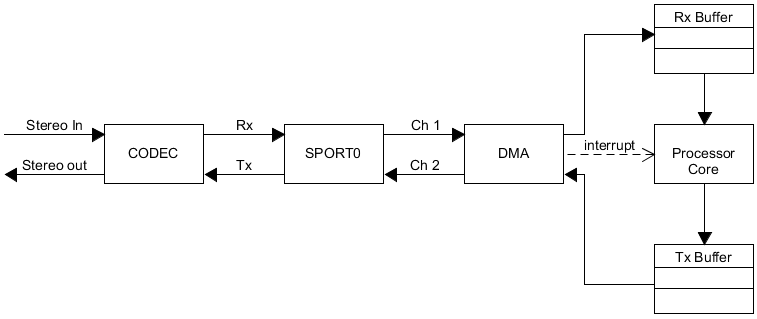
\includegraphics[width = 400pt]{Img/Struktur}
	\caption{Struktur NSS}
	\label{fig:LMS_filter}
\end{figure}

Igennem processen af vores funktionalitet, sendes lydsignalet gennem en codec1836, som har til opgave at sende inputtet gennem en ADC, hvorefter den sender det digitale signal videre til SPORT0, som står for at modtage og sende dataen. Igennem dette projekt bruger vi den interne clock, hvor frekvensen kan beregnes ud fra formlen:

\begin{figure}[H]
	\centering
	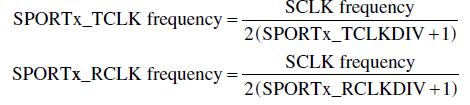
\includegraphics[width = 300pt]{Img/Frekvens}
	\caption{Formel for clock frekvens}
	\label{fig:clock_frek}
\end{figure}

DMA'en står for at sende dataen videre til Rx bufferen, når bufferen er fuld sender DMA'en interrupt til processeren om at procesere den modtagne data. \\
I den modsatte retning bliver det proceserede data flyttet til Tx bufferen, når Tx bufferen er fuld, sendes det til SPORT0 via DMA'en med Ch 2. Igen styres hastigheden af den interne clock frekvens, hvor hastigheden kan beregnes fra figur \ref{fig:clock_frek}. 
Til sidst bliver dataen samplet gennem CODEC, som konverterer til til et analogt signal vha. den en DAC.
  

\newpage

